\documentclass[11pt]{article}
\usepackage[textwidth=18.0cm, textheight=23.0cm, top=2.0cm]{geometry}
\usepackage{pst-all}
\usepackage{amssymb}
\usepackage{tikz}
\usepackage{underscore}\begin{document}
\pagestyle{empty}


ClassName: \underline{\textbf{Class_04.2bp-8}}
\par
BinSize: \underline{\textbf{100 × 100}}
\par
ReduceSize: \underline{\textbf{100 × 100}}
\par
TypeNum: \underline{\textbf{20}}
\par
Num: \underline{\textbf{20}}
\par
OutS: \underline{\textbf{10000}}
\par
InS: \underline{\textbf{6730}}
\par
Rate: \underline{\textbf{0.673}}
\par
UB: \underline{\textbf{1}}
\par
LB0: \underline{\textbf{1}}
\par
LB: \underline{\textbf{1}}
\par
LBWithCut: \underline{\textbf{1}}
\par
NodeCut: \underline{\textbf{0}}
\par
ExtendedNodeCnt: \underline{\textbf{1}}
\par
GenNodeCnt: \underline{\textbf{1}}
\par
PrimalNode: \underline{\textbf{0}}
\par
ColumnCount: \underline{\textbf{1}}
\par
TotalCutCount: \underline{\textbf{0}}
\par
RootCutCount: \underline{\textbf{0}}
\par
LPSolverCnt: \underline{\textbf{1}}
\par
PricingSolverCnt: \underline{\textbf{0}}
\par
BranchAndBoundNum: \underline{\textbf{1}}
\par
isOpt: \underline{\textbf{true}}
\par
TimeOnPrimal: \underline{\textbf{0.000 s}}
\par
TimeOnPricing: \underline{\textbf{0.000 s}}
\par
TimeOnRmp: \underline{\textbf{0.063 s}}
\par
TotalTime: \underline{\textbf{0.125 s}}
\par
\newpage


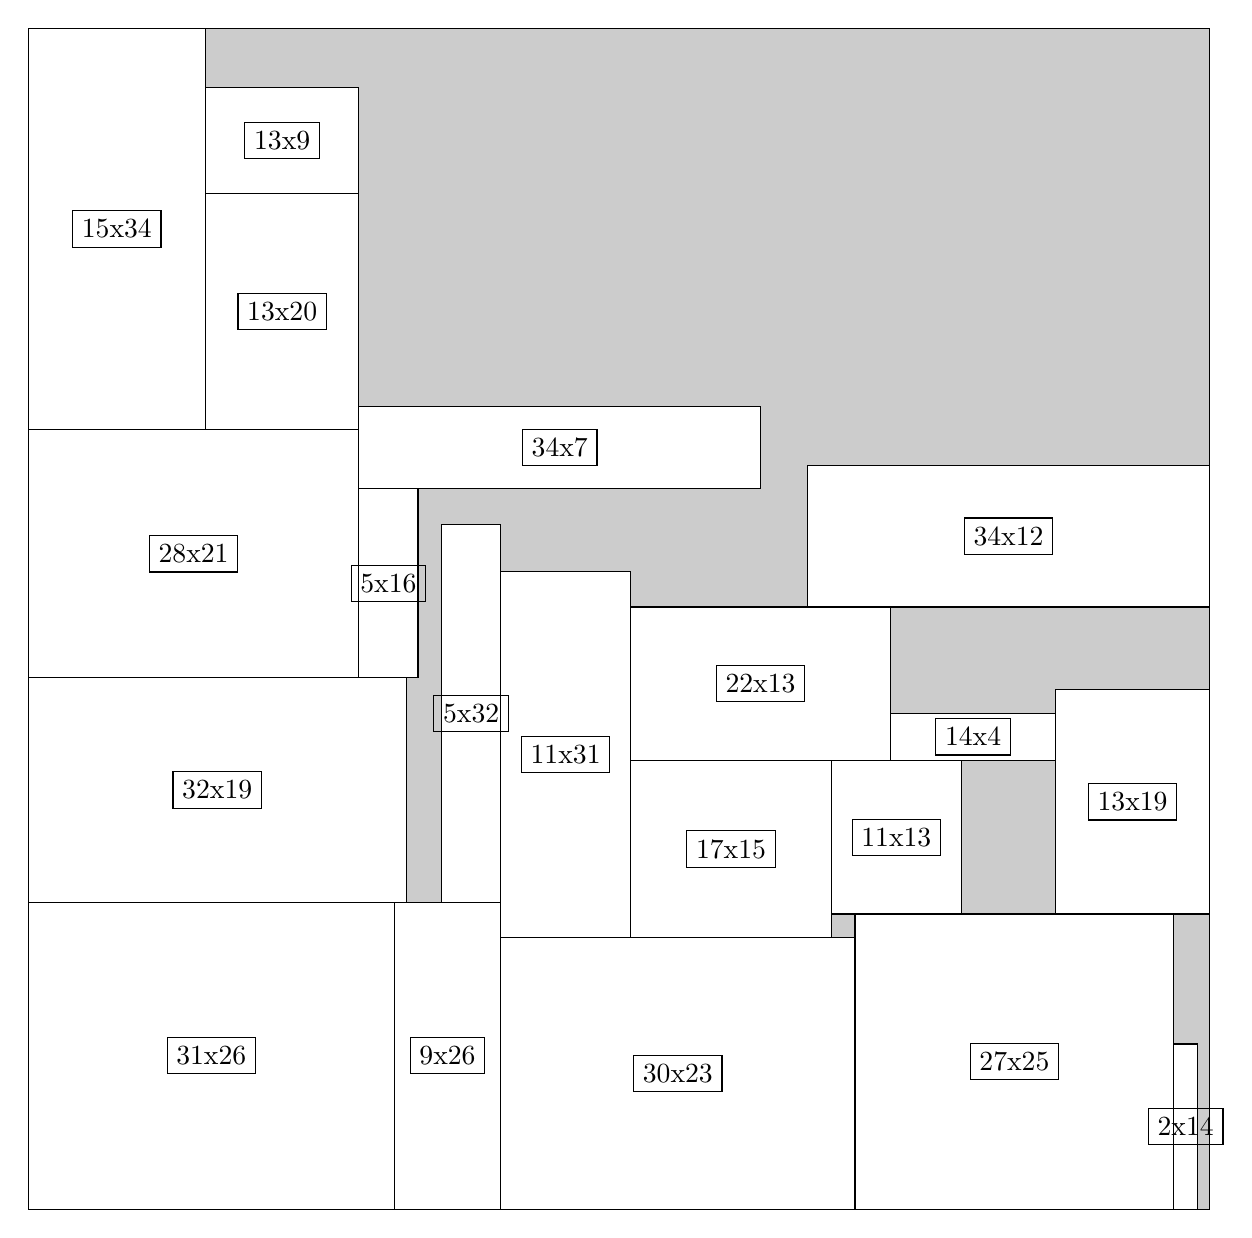
\begin{tikzpicture}[shorten >=1pt,scale=1.0,every node/.style={scale=1.0},->]
\tikzstyle{vertex}=[circle,fill=black!25,minimum size=14pt,inner sep=0pt]
\filldraw[fill=gray!40!white, draw=black] (0,0) rectangle (15.0,15.0);
\foreach \name/\x/\y/\w/\h in {31x26/0.0/0.0/4.6499999999999995/3.9,30x23/6.0/0.0/4.5/3.4499999999999997,27x25/10.5/0.0/4.05/3.75,32x19/0.0/3.9/4.8/2.85,28x21/0.0/6.75/4.2/3.15,2x14/14.549999999999999/0.0/0.3/2.1,34x12/9.9/7.6499999999999995/5.1/1.7999999999999998,11x31/6.0/3.4499999999999997/1.65/4.6499999999999995,22x13/7.6499999999999995/5.7/3.3/1.95,13x20/2.25/9.9/1.95/3.0,17x15/7.6499999999999995/3.4499999999999997/2.55/2.25,13x19/13.049999999999999/3.75/1.95/2.85,34x7/4.2/9.15/5.1/1.05,9x26/4.6499999999999995/0.0/1.3499999999999999/3.9,5x32/5.25/3.9/0.75/4.8,11x13/10.2/3.75/1.65/1.95,13x9/2.25/12.9/1.95/1.3499999999999999,5x16/4.2/6.75/0.75/2.4,14x4/10.95/5.7/2.1/0.6,15x34/0.0/9.9/2.25/5.1}
\filldraw[fill=white!40!white, draw=black] (\x,\y) rectangle node[draw] (\name) {\name} ++(\w,\h);
\end{tikzpicture}


w =31 , h =26 , x =0 , y =0 , v =806
\par
w =30 , h =23 , x =40 , y =0 , v =690
\par
w =27 , h =25 , x =70 , y =0 , v =675
\par
w =32 , h =19 , x =0 , y =26 , v =608
\par
w =28 , h =21 , x =0 , y =45 , v =588
\par
w =2 , h =14 , x =97 , y =0 , v =28
\par
w =34 , h =12 , x =66 , y =51 , v =408
\par
w =11 , h =31 , x =40 , y =23 , v =341
\par
w =22 , h =13 , x =51 , y =38 , v =286
\par
w =13 , h =20 , x =15 , y =66 , v =260
\par
w =17 , h =15 , x =51 , y =23 , v =255
\par
w =13 , h =19 , x =87 , y =25 , v =247
\par
w =34 , h =7 , x =28 , y =61 , v =238
\par
w =9 , h =26 , x =31 , y =0 , v =234
\par
w =5 , h =32 , x =35 , y =26 , v =160
\par
w =11 , h =13 , x =68 , y =25 , v =143
\par
w =13 , h =9 , x =15 , y =86 , v =117
\par
w =5 , h =16 , x =28 , y =45 , v =80
\par
w =14 , h =4 , x =73 , y =38 , v =56
\par
w =15 , h =34 , x =0 , y =66 , v =510
\par
\newpage


\end{document}